\documentclass{school-22.211-notes}
\date{May 22, 2012}

\begin{document}
\maketitle


\lecture{Exam 3 Review: Dynamics \& Kinetics}
\begin{enumerate}
\item Fission happens very quickly but depletion effects are felt on much longer time scales. 
  \begin{itemize}
    \item Fission: $\sim 10^{-12}$s. 
    \item Prompt neutron life time: $\sim 10^{-5 \sim -4}$s. 
    \item Temperature effects: fuel $\sim 10^{-2}$s, coolant $\sim 100$s. 
    \item Fuel depletion: Xe $\sim$ hours, Pu$\sim$ days, fuel depletion is on the order of months.
    \item Spent fuel decay: $\sim$ 1000s years. 
  \end{itemize}

\item Delayed neutrons concepts: 
  \begin{itemize}
  \item Dominant FP that emits delayed neutrons is Br-87: we use Br-87 with a 55.6s half-life to represent group 1 in 8-group model. 
  \item Burst vs. saturated measurement. Burst means prompt neutrons; saturated means total neutrons. 
  \item Delayed yields $\nu_d$ depend on: fissioning species, neutron energy ($E \up, \nu \up$). 
    \begin{itemize}
    \item Absolute yield: \# delayed neutrons per fission; unit: neutrons/fission. Know: \hi{U238 = 0.04, U235= 0.016.} \textbf{13 S904 Exam \#1}: What is the mean number of delayed neutrons emitted per U235 thermal fission? Answer: 0.016.  
    \item Relative yield: absolute yield of an isotope divided by total absolute yield by all isotopes; unit: percentage. 
    \end{itemize}

  \item Delayed neutron fraction $\beta = \frac{\nu_d}{\nu}$: \# delayed neutrons divided by total \# fission neutrons. Know: 
    \begin{itemize}
    \item U-235 thermal: $\beta = 0.0067$; Pu-239: thermal $\beta = 0.0022$ fast $\beta = 0.0020$\footnote{less delayed neutrons, could make control harder}; U-238: fast $\beta = 0.0164$. 
    \item We talk about $\beta_{\mathrm{effective}}$ that is weighted by flux. 
    \item $\beta$ can vary with BU, though the variations in BU are on a much larger time scale than usual range of application of PKEs. 
    \end{itemize}
    \begin{table}[h]
      \centering
      \begin{tabular}{|c|c|c|} \hline
        & $\nu_d$ (thermal/fast) & $\beta$ (thermal/fast) \\ \hline
        U-235 & 0.01668/0.01673 & 0.0067/0.0064 \\ \hline
        U-238 & -/0.046 & -/0.0164 \\ \hline
        Pu-239 & 0.0157/0.0152 & 0.0022/0.0020 \\ \hline
      \end{tabular}
    \end{table}


  \item Neutron emission spectra $\chi$: 
    \begin{itemize}
    \item Average neutron emission energy: \textbf{2 MeV} for prompt neutrons, \textbf{0.4 MeV} for delayed neutrons. Both spectrum are Maxwellian, except delayed neutrons are more thermal, which makes them more likely to fission. \textbf{13 S904 Exam \#2, \#3} asks for the mean emission energy of prompt and delayed neutrons from U235 thermal fission. 
    \item Strong energy dependency week isotope dependency: delayed neutron spectra vary very slightly for different fissioning nuclides, but very significantly on energy groups.
    \item Know U238 is extremely important for delayed neutrons. 
    \end{itemize}
  \end{itemize}

\item Know 8-group models: basically we don't have good theories to treat each isotope separately, thus we homogenize similar isotopes with one fixed decay constant (typically of the largest half-life in this group). 
\end{enumerate}

\clearpage
\topic{PKE Without Feedback}
\begin{enumerate}
\item Reactivity definitions: 
\begin{itemize}
  \item Static $\rho$ comes from steady-state transport equation, and it indicates excess (or lack) of reactivity present in the system. 
  \item Dynamic $\rho$ changes as a function of time and indicates changes from an initially stable system. 
    \eqn{ \rho(t) &= \frac{\keff - 1.0}{\keff} & \rho(t) &= \frac{\rho_f - \rho_i}{\rho_f} }
\end{itemize}
\begin{table}[ht]
  \centering
  \begin{tabular}{|c|c|c|} \hline
    Unit & Definition & Example \\ \hline
    $\Delta k$ & actual units of PKEs & 0.01 \\
    \% $\Delta k$ & & 1\% \\
    pcm & $10^5 \Delta k $ & 1000 pcm \\ \hline
    Dollars & $\frac{\Delta k}{\beta}$ & \$1.5 \\
    Cents & 100 Dollars & 150 cents \\ 
    Milli-beta & 1000 Dollars & 1500 milli-beta \\ \hline
  \end{tabular}
\end{table}

\item PKE assumptions: 
  \begin{itemize}
  \item Flux is separable $\phi(\vecr, E, t) = S(\vecr, E) T(t)$ ($S$ is the shape function, $T$ is the amplitude function). Classical PKE further assumes $S(\vecr, E)$ to remain constant with respect to $t$. 
  \item Assume no leakage, no external source of neutrons, no feedback. 
  \item Average properties, by integrate over all space and energy and normalize. 
  \item Classical PKE further assumes constant $\beta_i, \lambda_i$. 
  \item Minor: $\chi_p^j \to \chi_p, \beta^j \to \Sum_j \beta^j = \beta$ independent of fissioning species $j$; $\chi_d^i \to \chi_d$ independent of delayed neutron energy group $i$; $\beta (\vecr) \to \beta$ aka no spatial dependency. 
\end{itemize}

\item 2-group general PKE (dropped $\vecr$ for every term, and $t$ for $\Sigma, T, C$:
  \small
  \begin{align}
  \ddt \left[ T_1\right] &=   \int \dr  \phi_1^*  \left\{  - \Sigma_{r,1}  S_1 T_1  + (1-\beta) (\nu \Sigma_{f,1} S_{1}  T_{1} + \nu \Sigma_{f,2} S_2 T_2 ) \right\} + \int \dr \phi^*  \Sum_i \lambda_i C_i     \\
   \ddt \left[ T_2 \right] &=  
    \int \dr  \phi_2^*  \left[ - \Sigma_{a,2}  S_2 T_2 + \Sigma_{s12}  S_1 T_1  \right]   \\
   \ddt \left[ \int \dr C_i \right] &=   \int \dr \beta_i\left[ \nu \Sigma_{f,1} S_1 T_1 + \nu \Sigma_{f,2}  S_2  T_2 \right]   - \lambda_i \int \dr C_i 
  \end{align}
  \normalsize
  Implications:
  \begin{itemize}
  \item \textbf{$\rho(t)$ does not describe how much neutrons there are at a specific time; it describes how much neutrons there would be eventually.} 
  \item $\beta$ has no $T(t)$ temporal dependency. 
  \item $\beta$ only depends on $\phi_1^*$ but not $\phi_2^*$, because all delayed neutrons are born in group 1, hence we do not care about the neutron importance in group 2. 
  \item Similarly $\Lambda$ is the prompt neutron life time, thus only the importance of group 1 neutrons matters. 
  \end{itemize}

\item Classical PKE:
    \eqn{ \Aboxed{ \dTdt &= \frac{\rho- \Sum_i \beta_i }{\Lambda} T + \Sum_i \lambda_i C_i  + Q}  &  \Aboxed{ \ddt C_i &= \frac{\beta_i }{\Lambda} T - \lambda_i C_i }  }
    PKE parameters: 
    \eqn{ \rho(t) &= \frac{\expect{w, (F-M) \phi_0}}{\expect{w, F\phi_0}} & \Lambda &= \frac{\expect{w, v^{-1} \phi_0}}{\expect{w, F\phi_0}} & \beta_{\mathrm{eff}} &= \frac{\expect{w, F_d \phi_0}}{\expect{w, F \phi_0}}}
      \begin{enumerate}
      \item Reactivity $\rho$, where the top is the diffusion equation (or say the net production), and the bottom is fission rate if all neutrons show up instantaneously. $\displaystyle  \rho(t) = \frac{\nu \Sigma_f - \Sigma_a(1 + M^2 B_g^2)}{\nu \Sigma_f} = \frac{\keff - 1.0}{\keff},$ where $\keff = \frac{\frac{\nu \Sigma_f}{\Sigma_a}}{1 + M^2 B_g^2}$. 
        \scriptsize
        \begin{align}
          \rho (t) &= \frac{\int \bsp \dE \! \int \bsp \dr \Bigg\{ \!\divergence \! D  \gradient S  - \! \Sigma_t S  + \! \int \bsp \Sigma_s (\vecr \!, E' \bsp \to \bsp E, t) S \! \dE'   
            + \! \Sum_j \left( \! \chi_p^j (E) (1 \! - \! \beta^j) +  \! \Sum_i \chi_d^i (E) \beta_i^j \! \right) \! \int \bsp \nu \Sigma_f^j  S \dE'  }{\int \bsp \dE \int \bsp \dr \Sum_j \left( \chi_p^j (E) (1-\beta^j) + \Sum_i \chi_d^i (E) \beta_i^j \right) \int \bsp \nu \Sigma_f^j S \dE'} 
        \end{align}
        \normalsize

      \item The delayed neutron fraction (notice there is prompt neutron dependent $\chi_p^j(E)$ term in it). If ignore fissioning spectrum, $\beta \approx \Sum_i \beta_i$. 
        \begin{align}
          \beta_i (t) &= \frac{\int \bsp \dE \int \bsp \dr \left[ \Sum_j \chi_d^j (E) \beta^j \int_0^{\infty} \nu \Sigma_f^j (\vecr, E', t) S(\vecr, E') \dE' \right] }{\int \bsp \dE \int \bsp \dr \Sum_j \left( \chi_p^j (E) (1-\beta^j) + \Sum_i \chi_d^i (E) \beta_i^j \right) \int \bsp \nu \Sigma_f^j S \dE'} 
        \end{align}

      \item Prompt neutron lifetime, which is $\sim 1/v$ of shape divided by almost-instantenous-fission-rate. Know $\Lambda \sim 10^{-5}$ for LWRs; smaller for SFR, and larger for CANDU. 
\eqn{ \Lambda (t) = \frac{\int \bsp \dE \int \bsp  \dr \left[ \frac{1}{v} S(\vecr, E) \right] }{\int \bsp \dE \int \bsp \dr \Sum_j \left( \chi_p^j (E) (1-\beta^j) + \Sum_i \chi_d^i (E) \beta_i^j \right) \int \bsp \nu \Sigma_f^j S \dE'}  
\boxed{ \approx \frac{1}{v \nu \Sigma_f} \xrightarrow{\mathrm{criticality}} \frac{1}{v \Sigma_a} }   \notag }

      \item The $i$-th precursor, $C_i (t) = \int \dE \int \dr C_i (\vecr, t)$. The total external source, $Q(t) = \int \dE \int \dr Q (\vecr, t)$. 
      \end{enumerate}

%%%%%% Classical %%%%%



%%%%%%% %%%%%%%
\item Steady state solution of classical PKE: 
  \begin{align}
    \ddt C_i (0) &= 0  &\Rightarrow  C_i (0) &= \frac{\beta_i}{\Lambda \lambda_i} T_0  &  \ddt T(0) &= 0  &\Rightarrow \rho(0) &= 0  \label{in-hour}
  \end{align}

\item The matrix form of the 1st order ODE is (assuming three precursor groups, can be easily extend for more precursor groups),  
\begin{align}
N &= \left[ \begin{array}{c} T \\ C_1 \\ C_2 \\ C_3 \end{array} \right]  
& \ddt N(t) &= \left[ \begin{array}{cccc} 
\frac{\rho(t) - \beta}{\Lambda} & \lambda_1 & \lambda_2 & \lambda_3 \\
\frac{\beta_1}{\Lambda} & - \lambda_1 & & \\
\frac{\beta_2}{\Lambda} & & -\lambda_2 & \\
\frac{\beta_3}{\Lambda} & & & -\lambda_3 \end{array} \right] 
\left[ N(t) \right] 
\end{align}

\item Numerical examples: the interesting cases: 
  \begin{itemize}
  \item Instantaneous $\rho = 0.1 \beta$: reactor wants to response immediately, hence the jump, though it does not have enough delayed neutron to sustain that increase, so the power would increase for the rest of the way (curve up) till time constant reaches the longest precursor group (55s). 
  \item Insert rod for 2s, hold for 20s, re-position to original position. Power would stabilize again but not to the original value, b/c we are solving for an eigenvalue problem, and what the asymptotic power is depends on how we get there. 
  \item Super-prompt critical: power ascension very sensitive as $\rho \approx \beta$. When $\rho > \beta$, reactivity does not have to wait for the delayed neutrons and change happens instantaneously. 
  \end{itemize}

\item \textbf{Prompt-jump approximation}: assumptions: subcritical $\rho < \beta$ (the smaller $\rho$ is, the more accurate the approximation is), precursor population does not respond instantaneously ($C_i^+ = C_i^-$), prompt neutron changes negligible ($\left. \dTdt \right|_{t = 0^-} = 0, \left. \dTdt \right|_{t = 0^+} = 0$), no source. 
  \begin{align}
    \ddt T(t) &\approx 0 = \frac{\rho - \beta}{\Lambda} T(t) + \lambda C(t) = \frac{\rho- \beta}{\Lambda} T(0^+) + \frac{\beta}{\Lambda} T_0 \\
    \Aboxed{ \frac{T(0^+)}{T_0} &= \frac{\beta}{\beta - \rho} }
  \end{align}
  More general, if initial reactivity is not exactly zero (but small), $\displaystyle \frac{T_1}{T_0} = \frac{\beta - \rho_0}{\beta - \rho_1}$. 

\item In-hour equation: assume solutions take the form of, $T(t) \approx C_i (t) \approx e^{\omega t}$, plug into PKE. Basically if we know $\beta_i, \omega, \lambda_i$ we can find $\rho$. Know $\omega$ is typically small except super prompt critical when $\omega$ is huge. 
  \eqn{ \Aboxed{ \rho &= \omega \Lambda + \Sum_i \frac{\beta_i \omega}{\omega + \lambda_i}} }
  Issues:
  \begin{itemize}
  \item A small reactivity range such that ignoring feedback is valid. 
  \item In-hour assumes constant $\beta_i$ which is not very accurate for, e.g. we drive the control rod in the center of a core. 
  \item \textbf{Asymptotic periods $T_0 = \frac{1}{\omega}$}: we can only use Inhour equation for asymptotic period, that is, a stable condition indicated by a constant period. Thus to use Inhour equation, we have to make the reactor stable first. For any time dependent problem, we have to use the more general IK. 
  \end{itemize}

\item Inverse Kinetics Equation: 1st order ODE again. First given $T(t)$ we solve for the precursor concentration, using $[A] = \mathrm{diag}[\lambda_i], [Y(t)] = \frac{\mathrm{diag}[\beta_i]}{\Lambda} T(t)$. 
\eqn{ \Aboxed{ [C(t)] &= [e^{-At}][C_0] + [e^{-At}] [A]^{-1} \left( [e^{At}][Y(t)] - [Y_0] \right) } }
Then manipulating PKEs, we can get $\rho(t)$ in terms of $T(t), C(t)$, 
\begin{align}
\Aboxed{\rho(t) &= \frac{\Lambda}{T(t)} \ddt T(t) + \beta - \frac{\Lambda}{T(t)} \Sum_i \lambda_i C_i(t) - \frac{\Lambda}{T(t)} Q(t) } \\
\Aboxed{ \rho_n &= \frac{\Lambda}{T_n} \frac{T_n - T_{n-1}}{t_n - t_{n-1}} + \beta - \frac{\Lambda}{T_n} \Sum_i \lambda_i C_{i,n} - \frac{\Lambda}{T_n} Q_n } 
\end{align}
\end{enumerate}


\clearpage
\topic{PKE with Feedback}
\begin{enumerate}
\item Why model feedbacks? 
  \begin{itemize}
  \item Magnitude of flux/power very sensitive (can grow very quickly): without feedback power shoots up with an asymptotic period; with Doppler feedback, both the reactivity and power decreases before the rod is even fully inserted.   
  \item Safety analysis: fuel enthalpy at failure depends on BU so we need to model rod worth accurately for safety analysis. 
  \end{itemize}

\item Fuchs-Nordheim model for RIAs: nice for intuition
  \begin{enumerate}
    \item 3 assumptions: 
      \begin{itemize}
      \item $\rho \gg \beta$, ignore the delayed neutrons thus drop all $C_i(t)$; 
      \item rapid transient thus no heat transfer from the fuel: $T_{\mathrm{fuel}} = T_{\mathrm{fuel}}^0 + \frac{1}{C_p} \int P(t) \dt$; 
      \item Doppler coefficient independent of temperature: $\rho(t) = \rho_{\mathrm{rod}} - \alpha (T_{\mathrm{fuel}} - T_{\mathrm{fuel}}^0)$. 
      \end{itemize}
    \item First method to derive $P(t)$: $\frac{\dP}{\dT_{fuel}} = \frac{\dPdt}{\dTdt}$, integrate over temperature and get
      \eqn{ P(t) &= P_0 + \frac{1}{\Lambda} \left[ C_p (\rho_{rod} - \beta) T_{fuel} (t)  - \frac{\alpha C_p}{2} T^2_{fuel} (t) \right]  }
      At peak power, we set $\frac{\dP}{\dT_{fuel}} = 0$, 
      \begin{align}
        \Aboxed{ T_{fuel}^{peak} &= \frac{\rho_{rod} - \beta}{\alpha} }  &  \Aboxed{ P^{peak} &= P_0 + \frac{C_p (\rho_{rod} - \beta)^2}{2 \Lambda \alpha} }
      \end{align}

    \item Second method to derive $P(t)$: $\frac{\dP}{\drho} = \frac{\dPdt}{\drhodt}$, integrate over $\rho$, 
      \eqn{ P(t) = P_0 + \frac{C_p}{2\alpha} \left[ - (\rho(t) - \beta)^2 + (\rho_{\mathrm{rod}} - \beta)^2 \right]  }
      Assume the transient terminates when $P(t)$ returns to $P_0$, then $\rho_{end} = 2 \beta - \rho_{rod}$, 
      \eqn{ \Aboxed{ T_{fuel}^{end} &= \frac{2 (\rho_{rod} - \beta)}{\alpha} + T_{fuel}^0 } }

    \item Take-away messages:
      \begin{itemize}
      \item Peak fuel temperature is independent of neutron lifetime $\Lambda$ and heat capacity $C_p$. Peak temperatures are proportionally larger than core average. 
      \item Peak power $\propto \frac{C_p}{\Lambda}$; consequence: FRs with smaller $\Lambda$ would generate tons of heat rapidly. 
      \item $\Delta T_{fuel}^{end} = 2 \Delta T_{fuel}^{peak}$. Reason: power is symmetric around peak; temperature is integrated results. 
      \item Asymptotic fuel temperature is independent of: reactivity insertion rate, neutron lifetime, heat capacity. 
      \item F-N model is a good estimation because temperature is basically integrated power, hence the speed of reactivity insertion does not matter, it is the amount of reactivity inserted over time that matters. 
      \item Using PKEs with feedback, we demonstrate that reactivity change rate $\down$, the smaller the overshoot is. Though teh asymptotic results are independent of the reactivity change rate (as also seen in the F-N model). 
      \item A second peak in power is characteristic of slow insertion. 
      \end{itemize}
  \end{enumerate}

\item PKEs with simple feedback: 
  \begin{align}
    \ddt T_{\mathrm{fuel}} (t) &= a P(t) - b [T_{\mathrm{fuel}}(t) - T_{\mathrm{coolant}}(t)] \\
    \ddt T_{\mathrm{coolant}} (t) &= c [T_{\mathrm{fuel}}(t) - T_{\mathrm{coolant}} (t) ] - d [T_{\mathrm{coolant}} (t) - T_{\mathrm{inlet}} (t) ] 
  \end{align}

\item Transient feedback effects
  \begin{enumerate}
  \item Time constants: recall the asymptotic power decay time constant is just that of the longest precursor. 
  \item $< \beta$ insertion/withdrawal: power overshoot/undershoot is proportional to the reactivity change rate (rate $\down$, overshoot/undershoot $\down$), and the asymptotic value is independent of the reactivity change rate. 
  \item $> \beta$ insertion/withdrawal: power and temperature would turn around due to Doppler feedback. 
  \item Asymptotic temperature only depends on the reactivity change, not the change rate. 
  \end{enumerate}

  \item Problem with our neutronics model: not accurate for large spatial flux changes. Problem with our TH model: very huge diffusive property, would not predict any thermal shock behavior. 
\end{enumerate}

%%%%%%%%%%%%%%%%%% Nodal %%%%%%%%%%%%%%%%%%%%
\clearpage
\topic{Homogenization \& Dehomogenization} 
Nodal methods\footnote{weighted residual is not on the final}. The point of Nodal methods is that we can achieve high accuracy with large node size (compared with finite difference methods). We turn a 3D PDE into 3 1D ODE that are coupled through averaged transverse leakage terms. 
    \begin{align*}
      \boxed{ - \Sigma_{Dg}^x \frac{\derivative^2}{\dxi_x^2} \bar{\psi}_{gx} (\xi_x) + \Sigma_{rg} \bar{\psi}_{gx} (\xi_x) = \frac{1}{\keff} \chi_g \Sum_{g'=1}^G \nu \Sigma_{fg'} \bar{\psi}_{g'x} (\xi_x) + \Sum_{g'=1}^G \Sigma_{sg'g} \bar{\psi}_{g'x} (\xi_x) - L_{gy} (\xi_x) - L_{gz} (\xi_x) }    \\
   \boxed{ - \Sigma_{Dg}^y \frac{\derivative^2}{\dxi_y^2} \bar{\psi}_{gy} (\xi_y) + \Sigma_{rg} \bar{\psi}_{gy} (\xi_y) = \frac{1}{\keff} \chi_g \Sum_{g'=1}^G \nu \Sigma_{fg'} \bar{\psi}_{g'y} (\xi_y) + \Sum_{g'=1}^G \Sigma_{sg'g} \bar{\psi}_{g'y} (\xi_y) - L_{gz} (\xi_y) - L_{gx} (\xi_y) }  \\
     \boxed{ - \Sigma_{Dg}^z \frac{\derivative^2}{\dxi_z^2} \bar{\psi}_{gz} (\xi_z) + \Sigma_{rg} \bar{\psi}_{gz} (\xi_z) = \frac{1}{\keff} \chi_g \Sum_{g'=1}^G \nu \Sigma_{fg'} \bar{\psi}_{g'z} (\xi_z) + \Sum_{g'=1}^G \Sigma_{sg'g} \bar{\psi}_{g'z} (\xi_z) - L_{gx} (\xi_z) - L_{gy} (\xi_z) } 
    \end{align*}
  \begin{enumerate}
    \item NEM: expand $\bar{\psi}(\xi)$ by 4th order polynomial, 
          \eqn{ \bar{\psi}(\xi) = \Sum_{i=0}^4 a_i P_i (\xi) }

    \item Analytical: we solve 1D 2-group transerse-integrated diffusion equation, 
      \begin{align}
      -D_1 \frac{\derivative^2 \psi_1(x)}{\dx^2} + \Sigma_{r1} \psi_1(x) - \frac{1}{\keff} (\nu \Sigma_{f1} \psi_1 (x) + \nu \Sigma_{f2} \psi_2 (x) ) &= - L_1(x) \notag \\
      -D_2 \frac{\derivative^2 \psi_2(x)}{\dx^2} + \Sigma_{r2} \psi_2(x) - \Sigma_{12} \psi_1 (x) &= - L_2 (x)  \label{ANM-1}
    \end{align}
      We assume the solution is in the form of, 
      \eqn{ \psi_g (x) &= \hat{\psi}_g^H e^{iBx} + \psi_g^P(x) }
      such that $\dpsidxn2 = - B^2$. Plug in Eq.~\ref{ANM-1}, we get a system of two equations $[A] [\hat{\psi}^H] = 0$. For non-trival solution, we set det$[A] = 0$, thus getting a quadratic equation of $B^2$ that we can find the harmonic mode to be, 
      \eqn{ B_1^2&= b\left(-1 + \sqrt{1 - \frac{c}{b^2}} \right) = \left\{ \begin{array}{cc} > 0 & \kinf > \keff \\ < 0 & \kinf < \keff \end{array} \right. }
      and the harmonic mode to be, 
      \eqn{ B_2^2&=b\left(-1 - \sqrt{1 - \frac{c}{b^2}} \right) <0 }
      We need both modes because $B_1^2$ and $B_2^2$ are different. In this case fast group uses fundamental mode, thermal group uses harmonic mode, thus the solution is, 
      \eqn{ \left[ \begin{array}{c} \psi_1^H(x) \\ \psi_2^H (x) \end{array} \right] = \left[ \begin{array}{c} a_{11} \sin(B_1 x) + a_{12} \cos (B_1 x) \\ a_{21} \sinh(B_2 x) + a_{22} \cosh(B_2 x) \end{array} \right] =  \left[ \begin{array}{cc} r_1 & r_2 \\ 1 & 1 \end{array} \right] \left[ \begin{array}{c} a_{21} \sin(B_1 x) + a_{22} \cos (B_1 x) \\ a_{23} \sinh(B_2 x) + a_{24} \cosh(B_2 x) \end{array} \right] }
     where the fast-to-thermal flux ratio is defined as,
     \eqn{ r_m &= \frac{a_{11}}{a_{21}} = \frac{a_{12}}{a_{22}} = \frac{D_2 B_m^2 + \Sigma_{r2}}{\Sigma_{12}} }
     We know the particular solution from the $L$ terms. 

    \item SAMN: uses NEM for fast group, transverse integrated 1D diffusion equation for the thermal group. Approximate source with 4th order Legendre polynomial. Analytical solution of the thermal group is, 
      \eqn{ \psi_g(x) &= A \sinh(\kappa_g x) + B \cosh(\kappa_g x) + \Sum_{i=0}^4 c_i P_i \left(\frac{2x}{h}\right), &\kappa_g&=\sqrt{\frac{\Sigma_g}{D_g}} }
      That is, we have exponential homogeneous and polynomial particular solutions. 
  \end{enumerate}

\begin{enumerate}
\item Transverse-integration procedure
  \begin{enumerate}
    \item 3D to coupled 1D: we pick a direction of interest, perform integration within node over the plane normal to that direction, then devide by the planar area. For instance, the transverse leakage term is, 
          \eqn{ L_{gu}(\xi_x) &= \frac{1}{h_u} \left( \bar{J}_{gur}(\xi_x) - \bar{J}_{gul}(\xi_x) \right), & u &= y,z }
          where the line-averaged surface current is, 
          \eqn{ \bar{J}_{yr} (\xi_x) &= \int_0^1 J_y(\xi_x, 1, \xi_z) \dxi_z, &\bar{J}_{yl}(\xi_x) &= \int_0^1 J_y(\xi_x, 0, \xi_z) \dxi_z }
          \eqn{ \bar{J}_{zr} (\xi_x) &= \int_0^1 J_z(\xi_x, \xi_y, 1) \dxi_y, &\bar{J}_{zl}(\xi_x) &= \int_0^1 J_z(\xi_x, \xi_y,  0) \dxi_y }
          Flux distribution is not sensitive to transverse leakage shape, so we approximate transverse leakage with quadratic shape (2nd order polynomial): 
          \eqn{ L(\xi) = \bar{L} + l_1 P_1(\xi) + l_2 P_2(\xi) }
          and then use average TL conservation scheme to determine $l_1, l_2$. 
          
    \item Weighted residuals: in NEM, we have for each energy group 16 unknowns and 8 knowns, the rest 8 comes from weighted residual method: 
    \eqn{ \int_0^1 w(\xi) \left( -\Sigma_D \frac{\derivative}{\dxi^2} \psi(\xi) + \Sigma_r \psi(\xi) \right) \dxi = \int_0^1 w(\xi) \left( \frac{1}{\keff} \chi \psi(\xi) + S(\xi) - L(\xi) \right) \dxi }
    The closure relationship basically forces the $P_1, P_2$ integration to go to zero: 
    \eqn{ \int_0^1 P_1(\xi) \left( - \Sigma_D \frac{\derivative}{\dxi^2} \psi(\xi) + \Sigma_r \psi(\xi) - Q(\xi) \right) \dxi &= 0, & a_3 &= \frac{5 q_1 + 3 q_3 - 5 a_1 \Sigma_r}{3(60 \Sigma_D + \Sigma_r)} }
    \eqn{ \int_0^1 P_2(\xi) \left( - \Sigma_D \frac{\derivative}{\dxi^2} \psi(\xi) + \Sigma_r \psi(\xi) - Q(\xi) \right) \dxi &= 0, & a_4 &= \frac{-7 q_2 + 3 q_4 + 7 a_2 \Sigma_r}{420(\Sigma_D + 3\Sigma_r)} } 
  \end{enumerate}


%%%%%%%%%%%%%%%%%%% Homogenenization methods %%%%%%%%%%%%%%%%%%%%%%%%%%
\item Homogenization methods
  \begin{enumerate}
    \item \textbf{Discontinuity factors}: since the homogenized flux distribution in each node is affected by $D$, and the choice of the flux weighted $D$ is somewhat arbitrary, the interface fluxes can be different. We define DF: 
      \eqn{ f_{gi,j}^{u-} &= \frac{\phi_{gi,j}^u (u_l)}{\hat{\phi}_{gi,j}^u (u_l)}, &f_{gi,j}^{u+} &= \frac{\phi_{gi,j}^u (u_{l+1})}{\hat{\phi}_{gi,j}^u (u_{l+1})} }
      ADFs are the homogeneous analogy to the heterogeneous assembly calculation (which is calculating a single-node problem with zero net current BC). ADFs are simply ratios of the surface-averaged fluxes to the cell-averaged fluxes in the heterogeneous assembly calculation.

    \item Reflector modeling: 
      \begin{itemize}
      \item Using empiracal albedos to replace the baffle and reflector is bad because using flux-volume weighted cross section distribute the strong absorption xs over the entire region. 
      \item We use DFs because they are less spatially sensitive than albedos. It is advantagous in that DFs are chosen so that the nodal model wouold reproduce the net currents at the core/baffle interface and the net reaction rates in both the assembly and the homogenized baffle without explicitly representing the baffle. 
      \item Fast neutron leakage makes up for 90\% of all leakage, so leakage is insensitive to enrichment, burnup etc. 
      \end{itemize}
  \end{enumerate}

\item Pin power reconstruction
  \begin{enumerate}
    \item Form functions: we multiple homogeneous solution by the form function to get the heterogeneous solution. 
      \eqn{ \phi_g^{het} (x,y) &= \phi_g^{hom}(x,y) \phi_g^{SA} (x,y) }

    \item Corner point discontinuity factors. 
      \begin{itemize}
      \item Corner point fluxes are approximated by assuming that intra-nodal flux distributions are separable: 
        \eqn{ \phi_{g,i,j}(x,y) = \frac{\phi_{g,i,j} (x) \phi_{g,i,j} (y)}{\bar{\phi}_{g,i,j}} }
      \item Heterogeneous corner point flux has to be continuous. Thus we need corner point ratios that are analogous to DFs that can be obtained from the lattice calculations. 
      \item In general, the corner-point fluxes are determined by averaging the four estimates of the heterogeneous corner-point flux, 
        \eqn{ \phi_g^{het,cp} &= \frac{1}{4} \left[ \phi_{g,i,j}^{hom,cp} \phi_{g,i,j}^{fct,cp} + \phi_{g,i+1,j}^{hom,cp} \phi_{g,i+1,j}^{fct,cp} + \phi_{g,i,j+1}^{hom,cp} \phi_{g,i,j+1}^{fct,cp} + \phi_{g,i+1,j+1}^{hom,cp} \phi_{g,i+1,j+1}^{fct,cp} \right] }
      \item In order to satisfy the continuity conditions of reconstructed fluxes, the best-estimate homogeneous corner-point fluxes for each node are computed by, 
        \eqn{ \hat{\phi}_{g,i,j}^{hom,cp} = \frac{\phi_g^{het,cp}}{\phi_{g,i,j}^{fct,cp}} }
      \item  The reconstructed corner point fluxes are then continuous. \textbf{CP ratio is the corner point analogue of ADF for assembly edges.}
      \end{itemize}
  \end{enumerate}
  Side note: there are two entirely different problems. One is an eigenvalue problem, using homogenized cross section, and output $k$, and the flux computed would be continuous. The other is a fixed-source problem, using $\keff$ as input (hence $J$ at interface), and generate discontinuous flux. 
\end{enumerate}

\clearpage
\topic{Perturbation, Adjoint}
%%%%%%%%%%%%%%%%%%% Perturbation Theory %%%%%%%%%%%%%%%%%%%%%%%%%%
\begin{enumerate}
\item  First-Order Perturbation (FOP): the point is to solve for reactivity resulted from a perturbation without have to solving for the perturbed spatial flux. There are three sets of expressions, one for unperturbed forward problem, one for the unperturbed adjoint problem,
\eqn{ A_0 \psi_0 &= \frac{1}{k_0} M_0 \psi_0 &A_0^*\psi_0^* &= \frac{1}{k_0^*} M^* \psi_0^*  }
and a third set of perturbed forward problem, 
\eqn{ A \psi &= \frac{1}{k} M \psi \label{pertb3}}
FOP approximate the perturbed problem using, 
\eqn{ A &= A_0 + \delta A   &M &=M_0 + \delta M  &\psi &=\psi_0 + \delta \psi &k&=k_0+\delta k}
Plug the above approximation into Eq.~\ref{pertb3} and simplify, we reach the FOP which is 2nd order accurate, 
   \eqn{ \boxed{\delta \rho \approx \frac{\expect{\psi_0^*, \left( \frac{1}{k_0} \delta M - \delta A \right) \psi_0 }}{\expect{\psi_0^*, M_0 \psi_0}}  } }

\item Adjoint fluxes physical meaning: if we put a neutron at this place this energy, what is the probability it would cause fission.

  \item Balance equations:
    \begin{align}
      -\gradient D_g  \gradient \phi_g + \Sigma_{tg} \phi_g &= \chi_g \Sum_{g'=1}^G \nu \Sigma_{fg'}  \phi_{g'} + \Sum_{g'=1}^G \Sigma_{sg'\to g} \phi_{g'} \\
      -\gradient D_g  \gradient \phi_g^* + \Sigma_{tg}  \phi_g^* &= \nu \Sigma_{fg}  \Sum_{g'=1}^G  \chi_{g'} \phi_{g'}^*  + \Sum_{g'=1}^G \Sigma_{sg\to g'}  \phi_{g'}^*
    \end{align}

  \item For two group, infinite medium case, with effective downscatter only, 
    \begin{align}
      \left[ \begin{array}{cc}
          \Sigma_{a1} + \Sigma_{12} - \frac{1}{\kinf} \nu \Sigma_{f1} & - \frac{1}{\kinf} \nu \Sigma_{f2} \\
          - \Sigma_{12} & \Sigma_{a2} \end{array} \right] 
      \left[ \begin{array}{c}
          \phi_1 \\ \phi_2 \end{array} \right] &= 0  
      &\frac{\phi_2}{\phi_1} &= \frac{\Sigma_{12}}{\Sigma_{a2}}   \\
      \left[ \begin{array}{cc}
          \Sigma_{a1} + \Sigma_{12} - \frac{1}{\kinf^*} \nu \Sigma_{f1} & - \Sigma_{12} \\
          - \frac{1}{\kinf^*} \nu \Sigma_{f2} & \Sigma_{a2} \end{array} \right] 
      \left[ \begin{array}{c}
          \phi_1^* \\ \phi_2^* \end{array} \right] &= 0  
      &\frac{\phi_2^*}{\phi_1^*} &= \frac{\frac{1}{\kinf^*} \nu \Sigma_{f2}}{\Sigma_{a2}}  
    \end{align}
    where 
    \eqn{ \kinf^* = \kinf = \frac{\nu \Sigma_{f1} + \nu \Sigma_{f2} \frac{\Sigma_{12}}{\Sigma_{a2}} }{\Sigma_{a1} + \Sigma_{12}} } 
    In the above example, we effectively have $M \phi = 0, M^* \phi^* = 0$, and by definition, the adjoint of Hermitean conjugate of a mtatrix is just complex-conjugating each of its element and then transposing, 
    \eqn{ M^* = \left[ \begin{array}{cc} a_{11} & a_{12} \\ a_{21} & a_{22} \end{array} \right]^* = \left[ \begin{array}{cc} a_{11}^* & a_{12}^* \\ a_{21}^* & a_{22}^* \end{array} \right]^T = \left[ \begin{array}{cc} a_{11}^* & a_{21}^* \\ a_{12}^* & a_{22}^* \end{array} \right] }
 
  \item Boundary conditions: $\psi, \psi^*$ are any two functions satisfying the appropriate boundary and continuity conditions for the angular flux and adjoint flux. If $\psi(\vecr, \Omega, E) = 0$ for all $\hat{n} \cdot \Omegahat < 0$, then the adjoint satisfying $\psi^*(\vecr, \Omegahat, E) = 0$ for $\hat{n} \cdot \Omegahat > 0$. 


  \item Meaning:
    \begin{itemize}
    \item Fundamental mode solution: adjoint eigenvalue is the same as the real eigenvalue: $k^* = k$. 
    \item Adjoint flux is defined as the asymptotic increase in total neutron population of a critical reactor for a neutron introduced a phase space (position $r$, direction $\omega$, and energy $E$): 
      \eqn{\frac{N(\infty) - N_0}{Q} &= \psi^* (\vecr, \Omegahat, E)  }
    \end{itemize}

  \item Spectra: 
    \begin{itemize}
    \item The PWR spectrum: . 
    \item For a typical two group problem, the adjoint flux should have the same shape for the two groups, except the magnitude is offset by $\frac{\phi_2^*}{\phi_1^*}$. 
    \end{itemize}

\item Adjoint fluxes in kinetics parameters\footnote{In operating reactors, they measure the control rod worth; they are no better than the delayed spectra}
  \begin{enumerate}
  \item Delayed spectra: 10 times that of the prompt for up to 0.1 MeV; then approahces prompt until smaller than prompt spectrum for 1 MeV and above. 

  \item $\bar{I}$ is the ratio of the adjoint weighted delayed chi to prompt chi, and it has a value of about 0.97.
   \eqn{ \bar{I} = \frac{\expect{S_0^* (E), \chi_d (E)}}{\expect{S_0^*(E), \chi_p (E)}} }
  \end{enumerate}

\end{enumerate}

\clearpage
\topic{Past Problems}
\begin{enumerate}
  \item Qual 2012 \#3. 
  \begin{enumerate}
    \begin{figure}[ht]
      \centering
      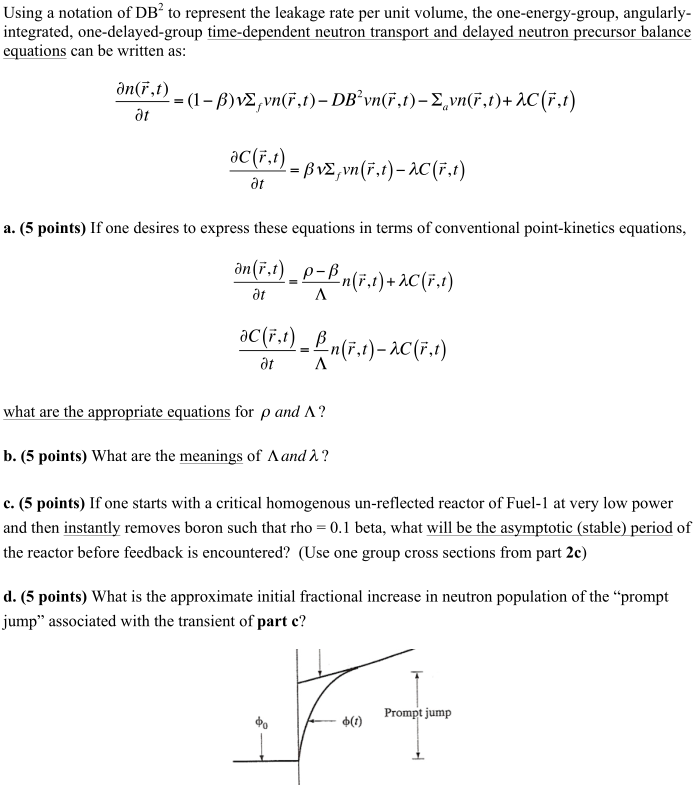
\includegraphics[width=6in]{images/qual/transient.png}
    \end{figure}
  \item $\displaystyle \rho = \frac{\keff - 1}{\keff}, \Lambda = \frac{1}{v \nu \Sigma_f}.
    $
  \item $\Lambda$ is prompt neutron lifetime, $\lambda$ is decay constant. 
  \item We use the inhour equation, and can ignore the $\omega \Lambda$ term can go away because $\Lambda$ is so small, 
    \eqn{ \rho &= \omega \Lambda + \Sum_i \frac{\beta_i \omega}{\omega + \lambda_i} \approx \Sum_i \frac{\beta_i \omega}{\omega + \lambda_i} }
    Because we only have one group cross section, 
    \eqn{ \rho = 0.1 \beta = \frac{\beta \omega}{\omega + \lambda}}
    where $\lambda = \frac{\ln 2}{\tau}$. Thus $\omega = 7.7 \times 10^{-3}, T = \frac{1}{\omega} = 130$s. 
  \item We use prompt jump approximation, 
    \eqn{ \frac{T(0^+)}{T_0} = \frac{\beta}{\beta - \rho} = \frac{\beta}{\beta - 0.1 \beta} = 1.111}

  \end{enumerate}
\end{enumerate}
%%%%%%%%%%%%%%%%%%%%%%%%% Final Exam End %%%%%%%%%%%%%%%%%%%%%%%%%%%%

\end{document}
